\documentclass[10pt]{beamer}

\usetheme{Unifesp}
\usepackage{thumbpdf,wasysym,ucs,pgf,pgfarrows,pgfnodes,pgfautomata,pgfheaps,
pgfshade,listings,multirow,xspace,amsmath}
\usepackage[utf8]{inputenc}
\lstset{language=[AspectJ]Java, stringstyle=\ttfamily,
basicstyle=\ttfamily, showstringspaces=false, commentstyle=\it}

\title[Pôster Gibis]{Pôster do Gibis}
\author[Fulano]{Fulano de Tal}
\institute{Instituto de Ciência e Tecnologia\\Universidade Federal de São Paulo}
\date{20 de Junho de 2015}
% \date{\vskip -0.5cm \tiny \flushright{\textit{Software systems are perhaps\\ the most intricate and complex\\ of the things humanity makes.\\ Fred Brooks}}}

\begin{document}

\frame{\titlepage}
\newcommand<>{\highlighton}[1]{%
  \alt#2{\structure{#1}}{{#1}}
}

\newcommand{\icon}[1]{\pgfimage[height=1em]{#1}}

%%%%%%%%%%%%%%%%%%%%%%%%%%%%%%%%%%%%%%%%%
%%%%%%%%%% Content starts here %%%%%%%%%%
%%%%%%%%%%%%%%%%%%%%%%%%%%%%%%%%%%%%%%%%%

\frame{ \tableofcontents }
\section{Introdução}
\subsection{O que é?}
\begin{frame}{O que é?}
	\begin{columns}[c]
		\column{.5\textwidth}
			\begin{figure}[h]
				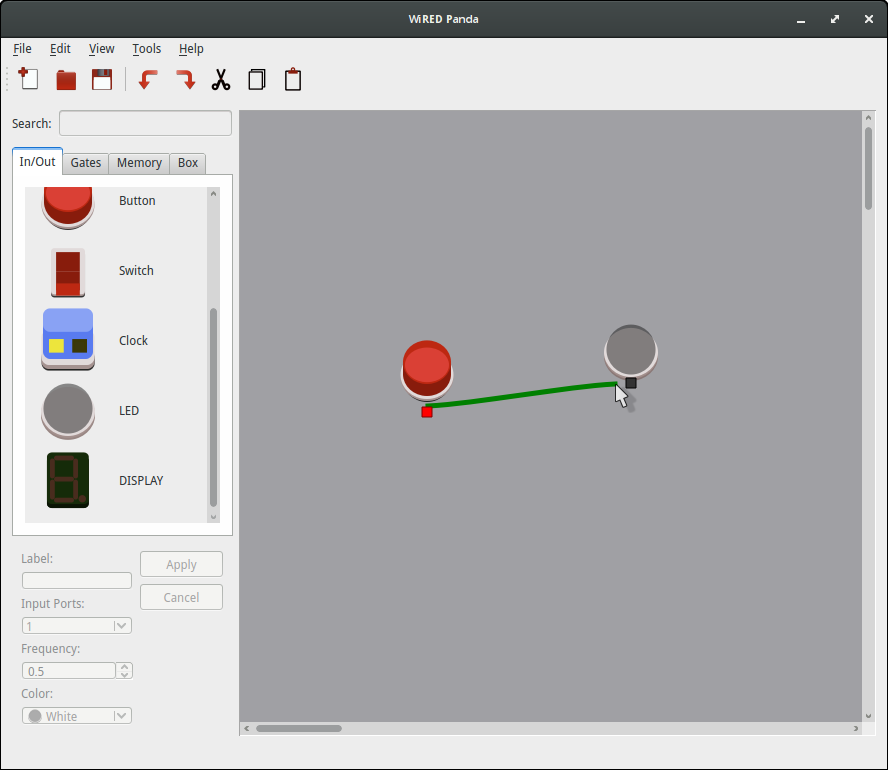
\includegraphics[width=1\linewidth]{./figures/cap01}
			\end{figure}
		\column{.5\textwidth}
			\textbf{WiRED PANDA} é um software didático para simulação de circuitos digitais.
	\end{columns}
\end{frame}

\end{document}
